\section{Estructura Interna Detallada de la Aplicación Móvil} 

La Figura \ref{fig:Diagrama_app_movil_detallado} profundiza en la arquitectura interna de la aplicación móvil, presentando los paquetes y componentes clave que la conforman. 

El punto de entrada principal de la aplicación es la actividad `MainActivity.kt`, la cual orquesta el flujo general de la aplicación. 

La interfaz de usuario de la aplicación se construye dentro del paquete `Pantallas`. Este paquete contiene las implementaciones de las pantallas de la aplicación utilizando Jetpack Compose. Cada pantalla se define mediante funciones Composable, que describen la estructura y el comportamiento de la interfaz de usuario de manera declarativa. 

La lógica y la gestión del estado de las `Pantallas` se encuentran en el paquete llamado `com.example.prueba3.Views`. Dentro de este paquete, los ViewModels actúan como intermediarios, proporcionando los datos necesarios a las Composables y manejando la lógica de las interacciones del usuario. Existe una relación directa entre las `Pantallas` y los `Views`, donde cada pantalla suele estar asociada a un ViewModel específico. 

El modelo de datos de la aplicación se define principalmente en el paquete `com.example.prueba3.Clases`. Este paquete contiene las clases que representan los datos utilizados por la aplicación. En su mayoría, estas clases son Data Classes, diseñadas para almacenar y transportar datos de manera concisa y eficiente.

La comunicación con los servicios backend se gestiona a través del paquete `RetroFit`. Este paquete contiene las interfaces de Retrofit que definen los endpoints de la API de los servidores remotos. Estas interfaces especifican las operaciones HTTP (GET, POST y DELETE) necesarias para interactuar con el Servidor Java Spring-Boot y el Servidor Red Neuronal. Retrofit se encarga de generar el código necesario para realizar estas solicitudes y procesar las respuestas del servidor.

\newpage

\begin{figure}[htbp!]
	\begin{center}
		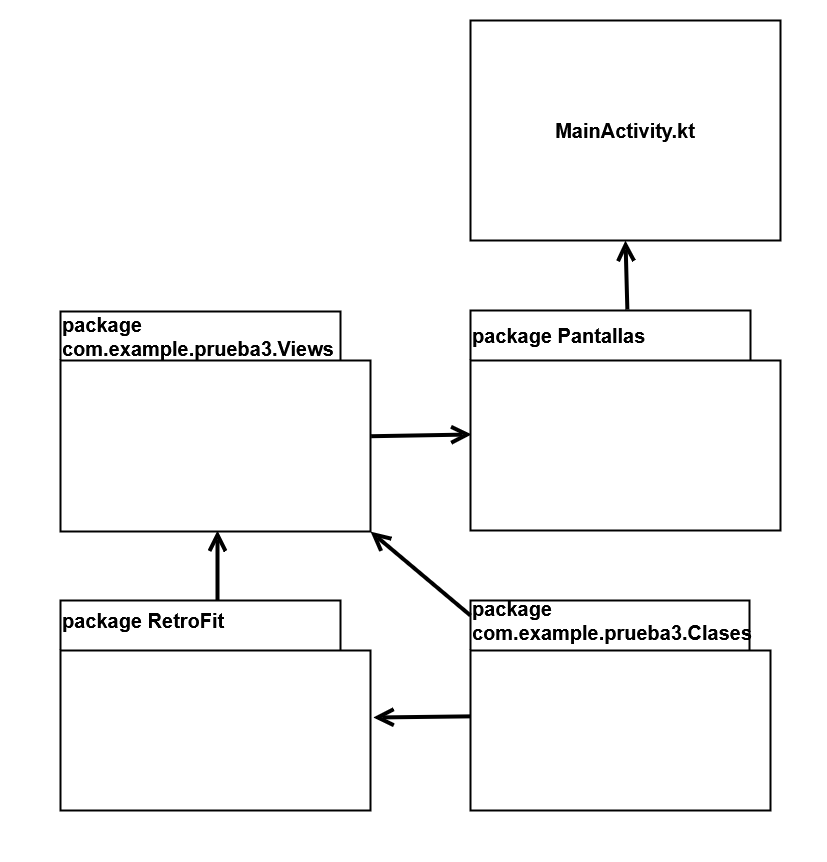
\includegraphics[width=0.6\textwidth]{DiagramasMoviles/DCM (1)}
		\caption{Estructura Interna Detallada de la Aplicación Móvil por Paquetes.}
		\label{fig:Diagrama_app_movil_detallado}
	\end{center}
\end{figure}



A continuación, se presentarán las clases contenidas en los paquetes `com.example.prueba3.Views` (ViewModels), `com.example.prueba3.Clases` (Data Classes) y las interfaces definidas en el paquete `RetroFit`, detallando su estructura y funcionalidad sección por sección. Adicionalmente, se incluirán diagramas de componentes específicos para cada una de las `Pantallas` de la aplicación móvil, ilustrando la composición de sus elementos y sus dependencias internas.

\newpage